\title{Warm-Up for $\pi+2$ Day, 2022}
\author{Dr. Jordan Hanson - Whittier College Dept. of Physics and Astronomy}
\date{\today}
\documentclass[12pt]{article}
\usepackage[a4paper, total={18cm, 27cm}]{geometry}
\usepackage{graphicx}
\usepackage{amsmath}
\usepackage{bm}
\def\rcurs{{\mbox{$\resizebox{.16in}{.08in}{
\includegraphics{ScriptR}}$}}}
\def\brcurs{{\mbox{$\resizebox{.16in}{.08in}{
\includegraphics{BoldR}}$}}}
\def\hrcurs{{\mbox{$\hat \brcurs$}}}
 
\begin{document}
\maketitle

\section{Memory Bank}

\begin{enumerate}
\item The dipole moment:
\begin{equation}
\mathbf{p} = \int \mathbf{r}' \rho(\mathbf{r}') d\tau' = \int \mathbf{r}' dq'
\end{equation}
\item The potential from the dipole term of the multipole expansion:
\begin{equation}
V_{\rm dipole}(\mathbf{r}) = \frac{1}{4\pi\epsilon_0} \frac{\mathbf{p} \cdot \hat{\mathbf{r}}}{r^2} \label{eq:2}
\end{equation}
\end{enumerate}

\section{Multipole Expansions}

\begin{enumerate}
\item Suppose there is a line charge along the $\hat{z}$-direction, with density $\pm\lambda$.  For a length $L/2$ below the origin, the density is $-\lambda$, and for a length $L/2$ above the origin, the density is $+\lambda$.  (a) Find the dipole moment, $\mathbf{p}$.  (b) Insert $\mathbf{p}$ into Eq. \ref{eq:2} to find the potential. (c) Calculate the $\mathbf{E}$-field.  Is the result resonable?  Why doesn't the field limit to something like $\approx Q/r^2$?
\end{enumerate}

\begin{figure}
\centering
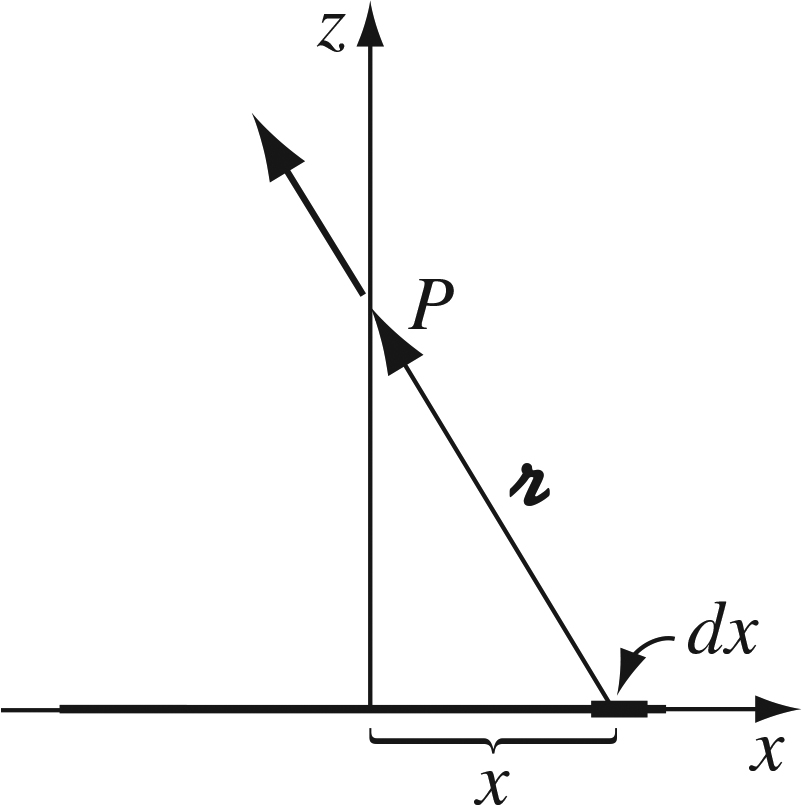
\includegraphics[width=0.25\textwidth]{figures/2_6.jpg}
\caption{\label{fig:1} Suppose there is a positive line charge to the right, and a negative line charge to the left.  \textit{Assume the charge distribution is along the $\hat{z}$-direction, not the $\hat{x}$-direciton.}}
\end{figure}

\end{document}